\setchapterstyle{kao}
\setchapterpreamble[u]{\margintoc}

\chapter{Practice and Measurements} % How it actually works
\labch{tc-practice-and-measurements}

\section{Tuning the Secondary Coil}\label{TC-tuningTheSecondary}

Tuning the secondary coil to the correct frequency is essential because all calculated values from section \ref{subsec:designing-the-secondary-coil} are highly idealized. For example, equation \ref{eq-parasitic-capacitance} is said to have a standard deviation of \(\sigma_{CL} \text{ in } \\pF = 3.6 \cdot D\), which leads to a standard deviation of around \(116\,kHz\) of the coil's resonant frequency. In addition, the relative permeability and permittivity of the carrier material is not taken into consideration in the calculations.

The coil was tuned by exciting the base of the secondary coil with a sinusoidal voltage. An oscilloscope probe, formed into a current loop, was placed near the top of the coil. The closer the excitation frequency was to the coil's resonant frequency, the higher the measured voltage on the oscilloscope. The frequency at which the measured voltage was at its maximum was the resonant frequency of the coil. By adding or removing windings, the resonant frequency could be lowered or raised until it exactly matched \(4\,MHz\).

In order to avoid adding windings, which is more tedious than removing them, the coil was initially wound \(120\,mm\) long, which is \(8\,mm\) longer than calculated. After going through the procedure of sweeping through all frequencies close to \(4\,MHz\), finding out the exact resonant frequency, and tuning it slightly towards the correct value over and over again, the final length turned out to be \(113\,mm\). This corresponds to a deviation of only 0.9\% from the calculation.

\section{The Class-E Stage}

The class-E amplifier was by far the trickiest part to get running. It took about seven months from the official project start and four prototypes to get first results.

In the first prototype, it was attempted to design the class-E amplifier using the design equations mentioned in section \ref{subsec:the-design-process}. The Tesla coil was converted into a single impedance value and seen as part of the load network. The calculated value for the capacitor \(C_2\) was already contained in this value, so it was simply left out. Guaranteed failure predicted by the simulation was simply ignored. In fact, without the DC-blocking capacitor, the whole amplifier looked like a short for direct current and the network had no chance to start oscillating.

First, it was assumed that this could be solved by reducing the noise in the PCB with a ground plane, which finally was not the solution.

The third design finally solved this problem by adding a \(100\,nF\) capacitor, but soon, another issue was discovered. The \(4\,MHz\) signal was still coming from a signal generator connected via a coaxial cable. Even though the Tesla coil did not create any arcs yet, it still produced an electromagnetic field. This field induced a voltage in the long cable from the signal generator and, after being amplified by the MOSFET driver, turned on the MOSFET when it should have been off.

Initially, this was believed to be black magic, but the fourth design tackled this flaw by adding the previously described \gls{vco} very close to the MOSFET driver. With some tweaking, it was able to produce arcs, even without any help from a grounded object.

The next step was to involve the interrupter signal. The first design did not use a latch, but two NPN transistors, which form an AND gate. This does, of course, not take care of the synchronization between the interrupter and base signal. Another bad decision was using current-driven transistors, which usually need to be handled with care in logic circuits. Even though the calculated resistor values seemed to be correct, the VCO always broke because the base of the connected transistor apparently drew too much current.

The signal synchronization and current issues were fixed by the sixth and final design. Its schematic corresponds to the one derived in chapter \ref{ch:design-and-simulation}. When operated in continuous mode by tying the interrupter signal to \(V_{CC}\), the coil behaved just like expected. In interrupted mode, the coil was able to play a single, if not only very distorted, frequency. Unfortunately, due to time constraints, this was as far as it got and the project had to be put temporarily on hold.

\subsection{Fine-Tuning the Setup} % Or Fine-tuning?

It is very unlikely that a class-E Tesla coil\sidenotes{And this is true for almost any Tesla coil} can achieve a stable operation on the first try. There are many different parameters that influence the behavior of the coil, but three have been found to have a major impact.

\subsubsection{Number of Primary Windings}

The turns ratio of a transformer is one of its most important properties, and a Tesla transformer is no exception. With only ten turns, adding or removing a winding greatly affects the primary coil's inductivity as well as the transformer's coupling factor. This relationship has been simulated in \texttt{EleFAnT2D} and is portrayed in figure \ref{fig:tuning-the-primary}.

\begin{figure}[h!]
    \centering
    \resizebox{0.7\textwidth}{!}{
    \begin{tikzpicture}
      \begin{axis}[
        axis y line* = right,
        y filter/.code=\pgfmathparse{#1 * 1000000},
        ylabel = \(L_P\) in \(\mu H\),
        xlabel = Number of Turns,
        ymin = 1.3,
        ymax=12,
        grid=both
        ]
        \addplot+[black!80, smooth, mark options={black!90}, mark=o] table[x=n,y=l,col sep=comma]{simon/resources/turns.csv};\label{{plot:lp}}
      \end{axis}
      \begin{axis}[
        axis y line* = left,
        xtick = {-1},
        ylabel = \(k\) in \(\%\),
        ymin=17.33,
        ymax=18.4,
        legend pos=north west,
        ]
      \addplot+[black!80, smooth, mark options={black!90}, mark=square] table[x=n,y=k,col sep=comma]{simon/resources/turns.csv};
      \addlegendentry{\(k\)};
      \addlegendimage{mark=o,/pgfplots/refstyle=plot:lp}\addlegendentry{\(L_P\)};
      \end{axis}
    \end{tikzpicture}}
    \caption{Tuning the Primary}
    \label{fig:tuning-the-primary}
\end{figure}

It has been shown that using between \(7\) and \(8.5\) windings yielded the best results. With \(10\) windings, the amplifier does run stable but cannot produce enough output power to create an arc.

\subsubsection{Operating Frequency}

As already observed in simulations, the overall efficiency falls drastically as the operating frequency diverges from the secondary coil's resonant frequency. With the ability to change the frequency generated by the \texttt{LTC1799} while the coil is running, it was relatively easy to determine the optimal frequency for each setup. In almost all cases, it was located somewhere between \(3.7\,MHz\) and \(3.95\,MHz\).

\subsubsection{Supply Voltage}

One last thing whose impact impact on the coil's output power was bigger than expected was the supply voltage. While in theory, the output power should be proportional to the square of the voltage, raising \(V_{CC}\) from \(50\,V\) to \(54\,V\) roughly doubled the maximum stable arc length.


\subsection{Measurements}

In the earlier prototypes, it was always important to monitor the MOSFET's gate signal. For one, to confirm that the signal generation worked as intended and for another, to measure the current operating frequency. Figure \ref{fig:gate-measured} shows the gate signal for a frequency of \(3.85\,MHz\).

\begin{figure}[h!]
    \centering
    \begin{tikzpicture}
      \begin{axis}[
        ylabel = \(V_{GS}\) in \(V\),
        x filter/.code=\pgfmathparse{#1 * 1000000000},
        xlabel = \(t\) in \(ns\),
        %ytick= {-5,0,5},
        %ymajorgrids,
        grid=both,
        xmin=0, xmax=600,
        extra y ticks={12},
        height=6cm,
        width=0.95\textwidth
        ]
        \addplot+[rounded corners=.5pt, black!80] table[x=t,y=v,col sep=comma, mark=none]{simon/resources/mosfet_gate_measured.csv};
      \end{axis}
    \end{tikzpicture}
    \caption{MOSFET Gate Signal}
    \label{fig:gate-measured}
\end{figure}

\newpage
Even while the Tesla coil was operating and generating arcs, it was not directly obvious whether the class-E amplifier operated in a stable manner or if the MOSFET could break any moment. Therefore it was crucial to be able to keep a look at the voltages in the circuit, especially \(V_{DS}\). If the drain-source voltage was either clipped, did not return to zero before turn-on, or looked problematic in any other way, it was safer to quickly turn off the Tesla coil and look for potential issues. Figure \ref{fig:vds-50} shows the \(V_{DS}\) with a supply voltage of \(50\,V\) and an operating frequency of \(3.85\,MHz\).

\begin{figure}[h!]
    \centering
    \resizebox{0.8\textwidth}{!}{
    \begin{tikzpicture}
      \begin{axis}[
        ylabel = \(V_{SC}\) in \(V\),
        x filter/.code=\pgfmathparse{#1 * 1000000000},
        xlabel = \(t\) in \(ns\),
        grid=both
        ]
        \addplot+[black!80] table[x=t,y=v,col sep=comma, mark=none]{simon/resources/mosfet_drain_measured.csv};
      \end{axis}
    \end{tikzpicture}}
    \caption{\(V_{DS}\) at \(50\,V\) and \(3.85\,MHz\)}
    \label{fig:vds-50}
\end{figure}

As already mentioned, increasing the supply voltage to the indented \(54\,V\) clearly increased the output power, but it also pushed the MOSFET to its limits, as shown in figure \ref{fig:vds-54}. This can be seen by the abrupt drop of the second and third half-wave. Also, the ringing after turn-on and the different heights of the voltage peaks are a clear indicator that the amplifier is not running ideally.

\begin{figure}[h!]
    \centering
    \resizebox{0.8\textwidth}{!}{
    \begin{tikzpicture}
      \begin{axis}[
        ylabel = \(V_{SC}\) in \(V\),
        x filter/.code=\pgfmathparse{#1 * 1000000000},
        xlabel = \(t\) in \(ns\),
        grid=both
        ]
        \addplot+[black!80] table[x=t,y=v,col sep=comma, mark=none]{simon/resources/mosfet_drain_measured54.csv};
      \end{axis}
    \end{tikzpicture}}
    \caption{\(V_{DS}\) at \(54\,V\) and \(3.85\,MHz\)}
    \label{fig:vds-54}
\end{figure}

\newpage
\section{Image Gallery}

\begin{figure}[h!]
    \centering
    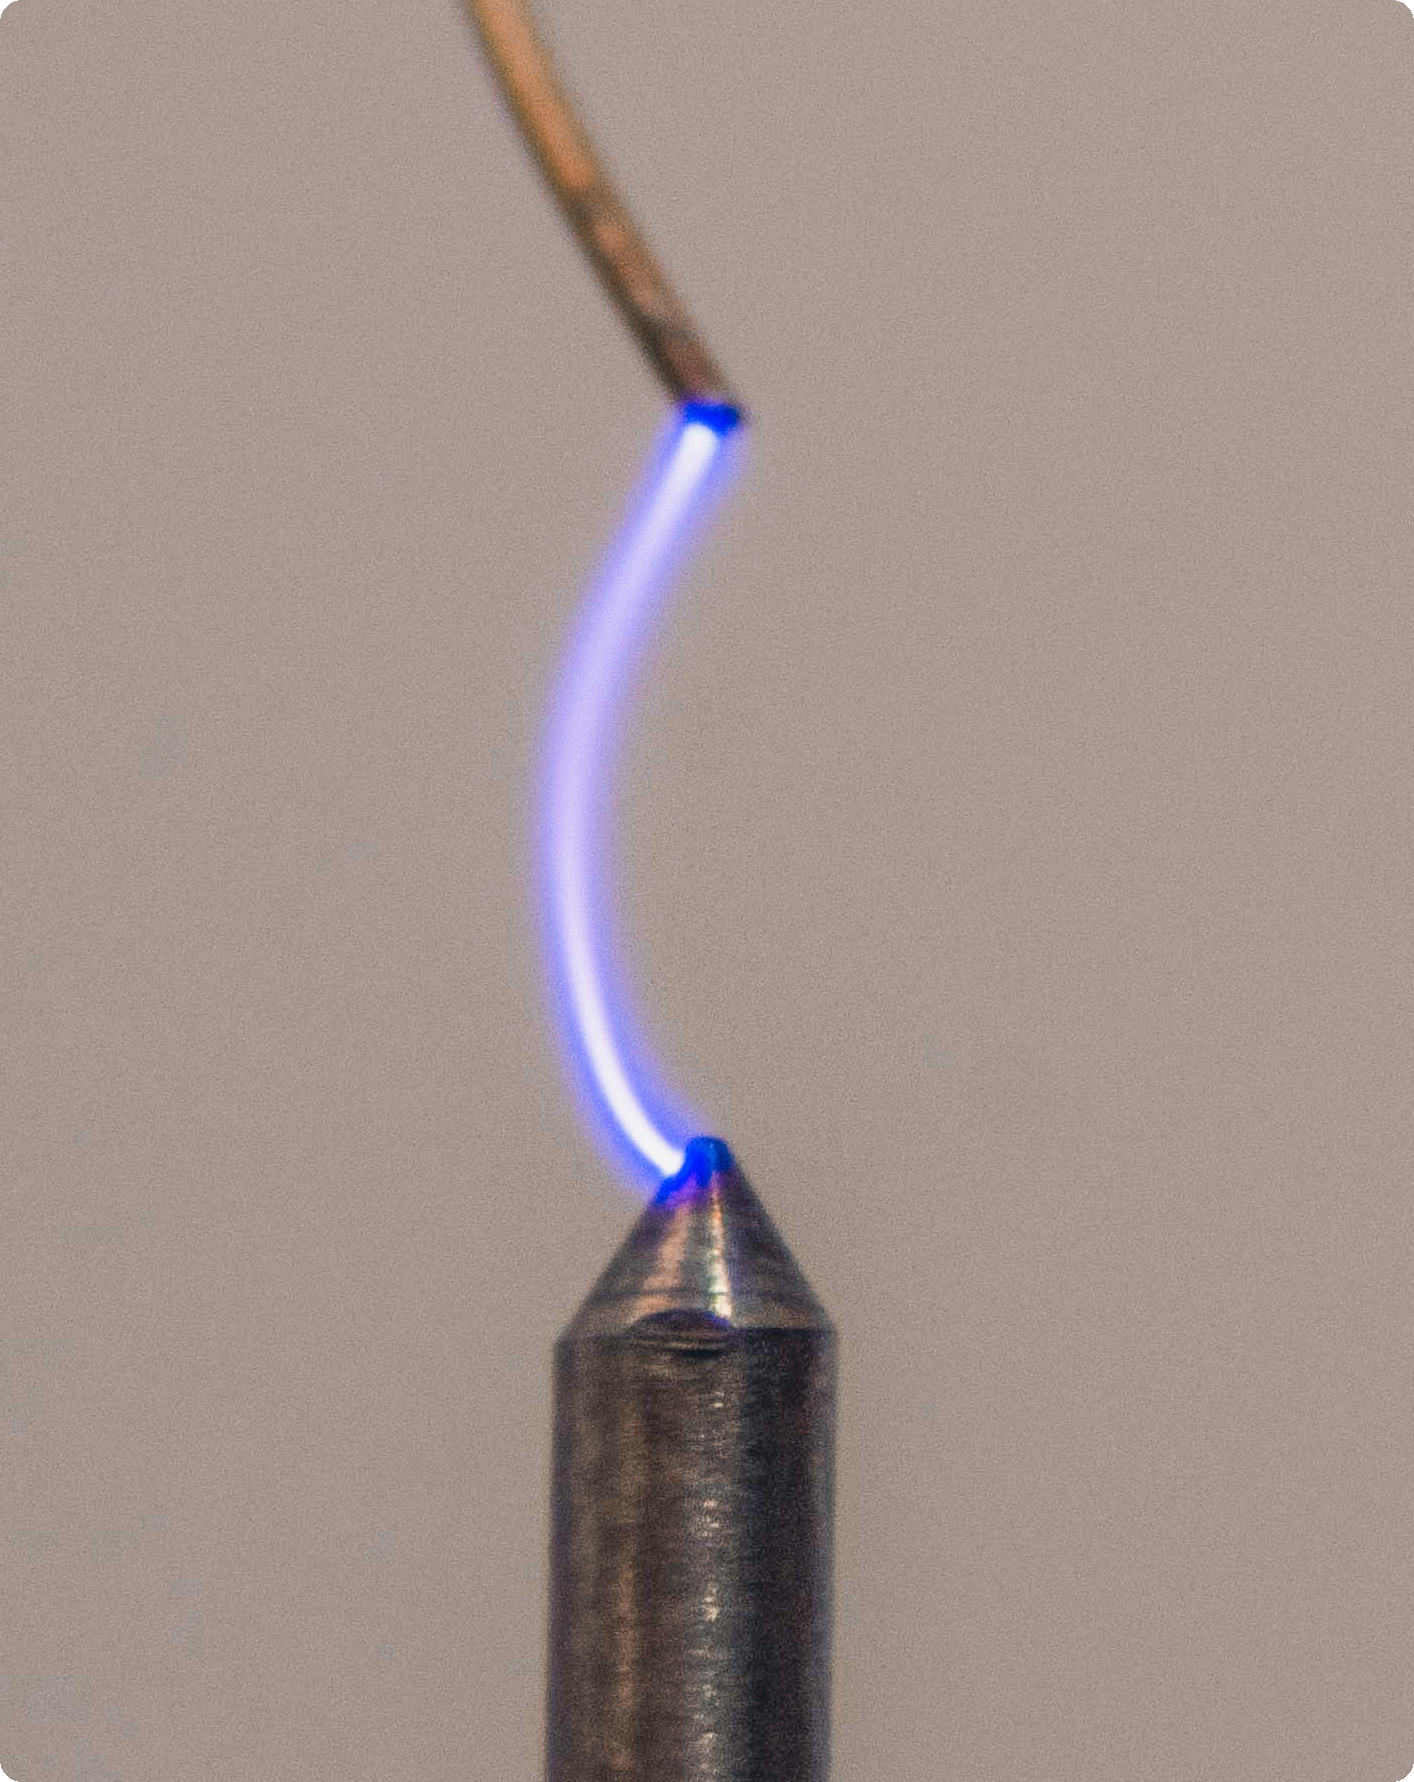
\includegraphics[width=0.7\textwidth]{simon/resources/blitzi1.jpg}
    \caption{Close-Up of the Arc}
    \label{fig:arc-closeup}
\end{figure}

\begin{figure}[h!]
    \centering
    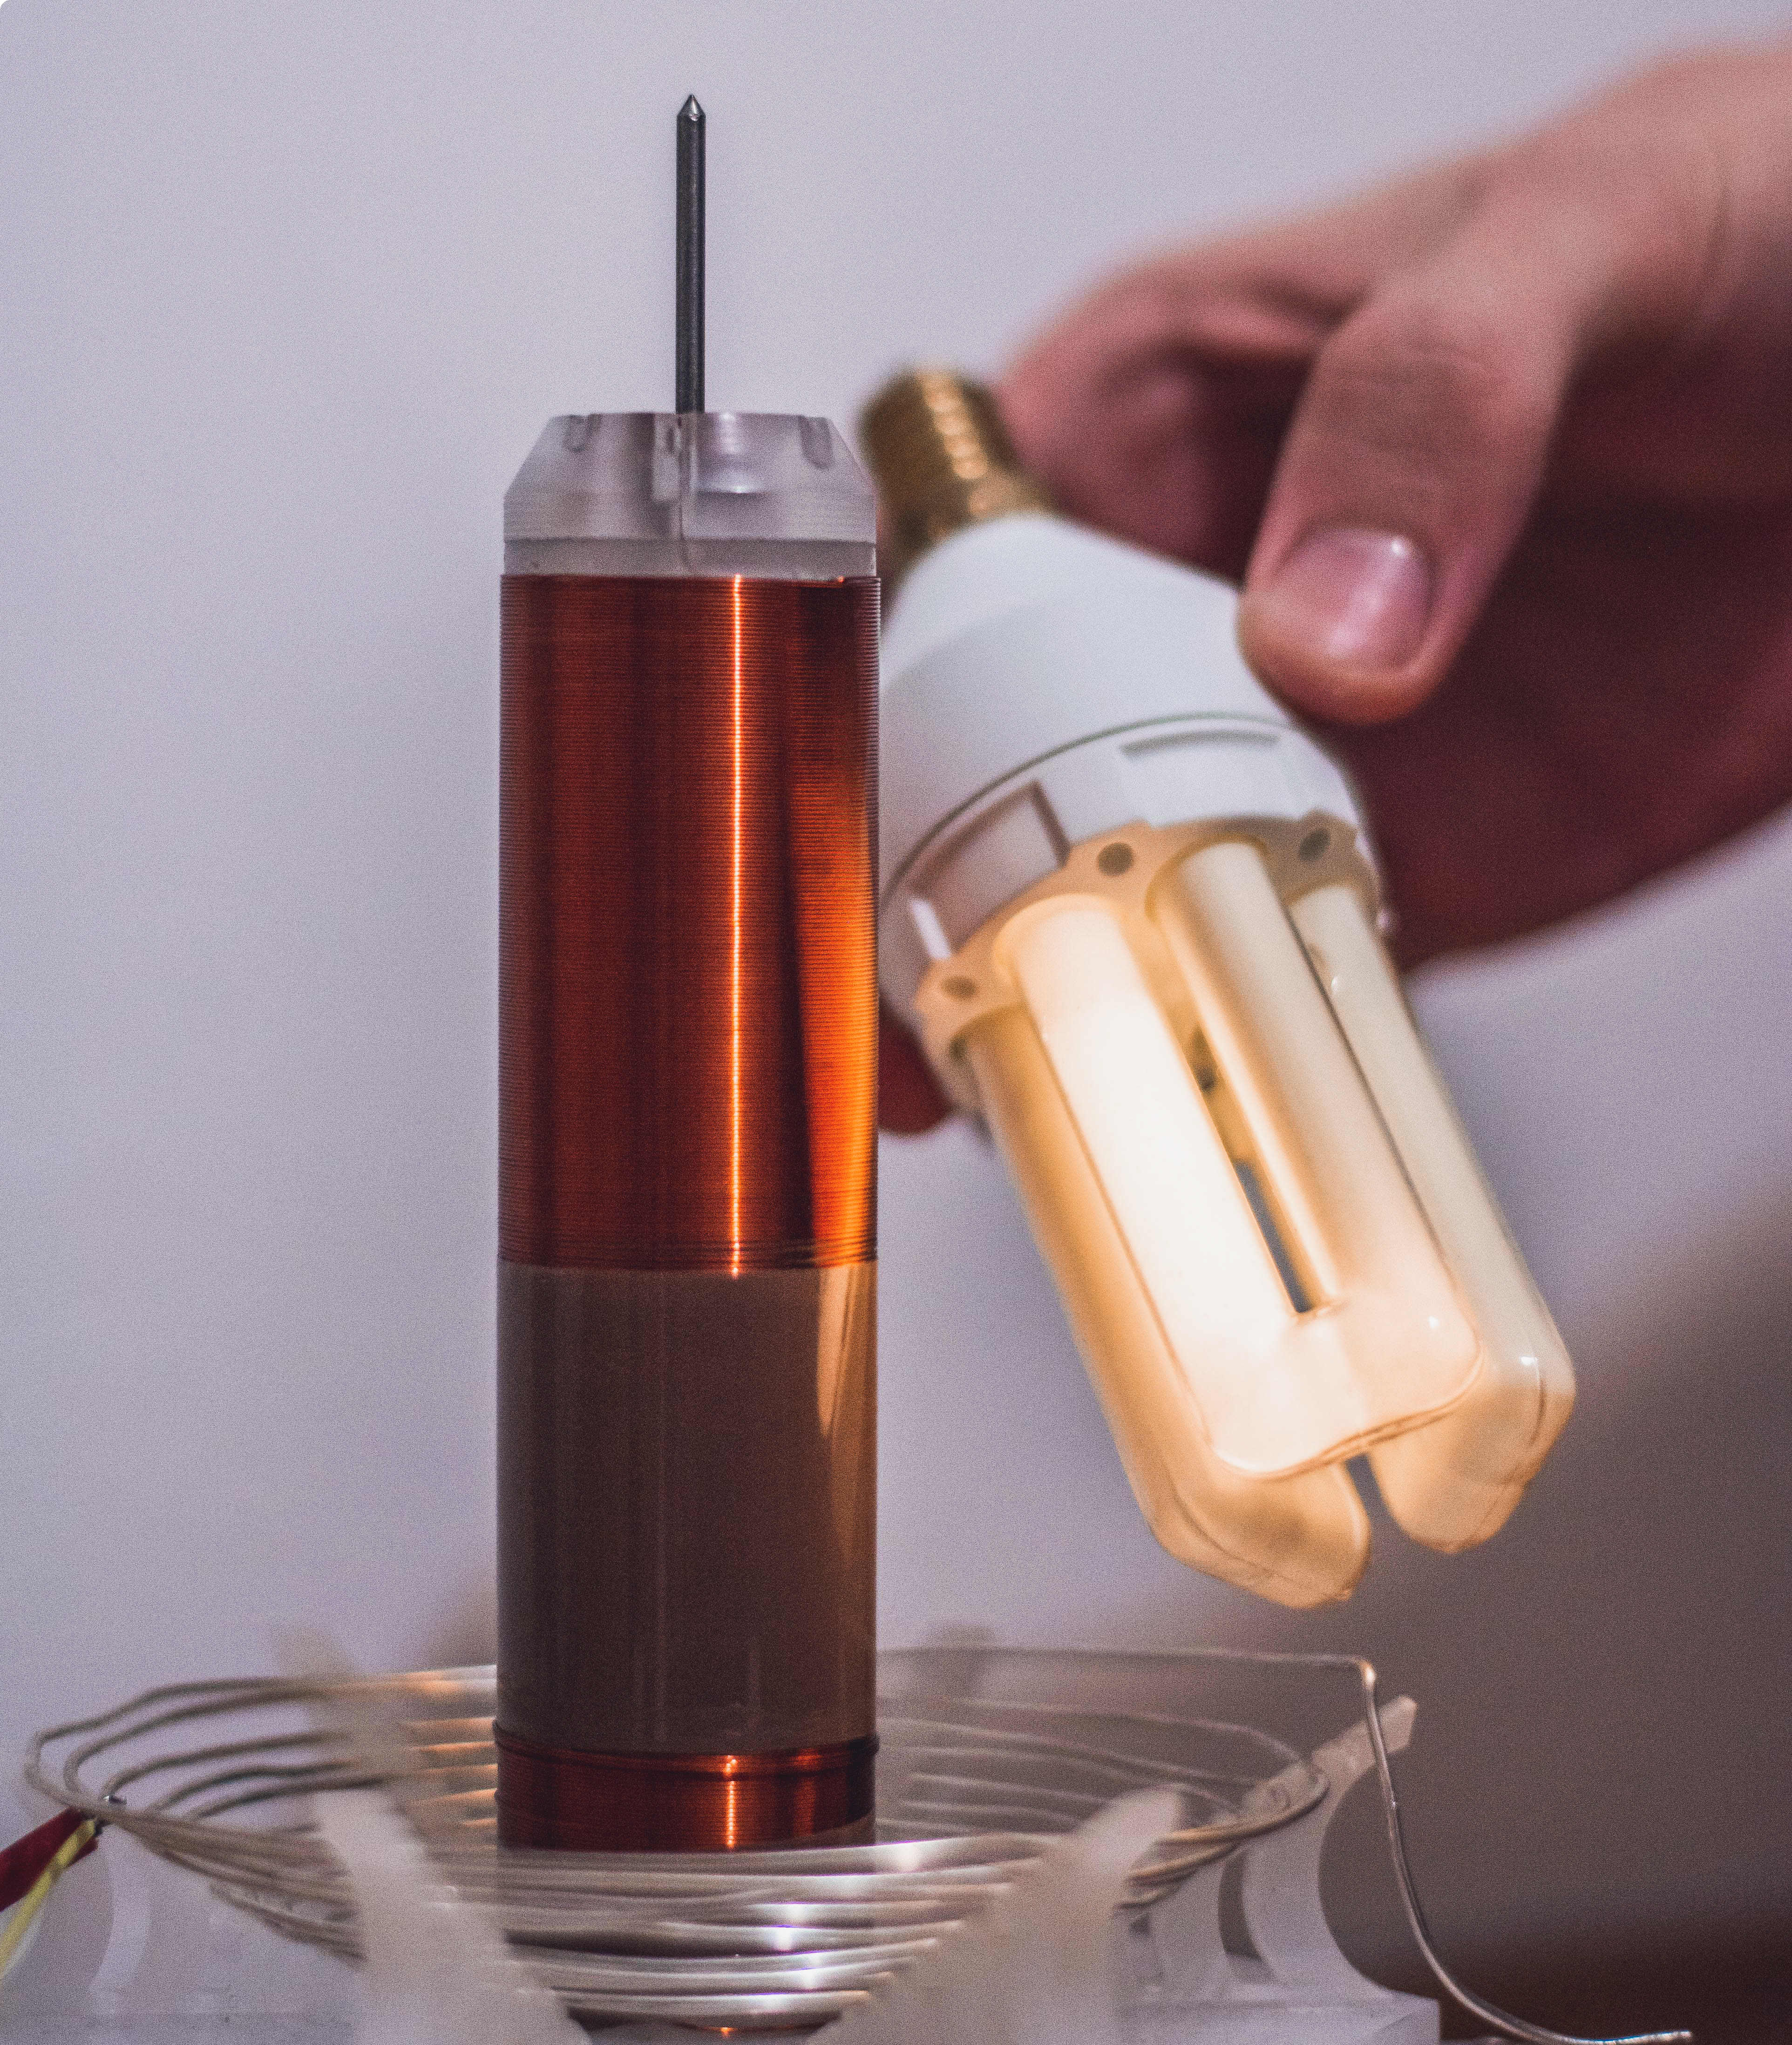
\includegraphics[width=0.7\textwidth]{simon/resources/blitzi2.jpg}
    \caption{Lighting a Lamp Wirelessly}
    \label{fig:lamp}
\end{figure}